\documentclass{article}
% set margins
\usepackage[left=1.5in, right=1in, top=1in, bottom=1in]{geometry}
% add spacing
\usepackage{setspace}
% use biblatex
\usepackage[style=numeric]{biblatex}
% add the bibliography
\addbibresource{bibliography.bib}
% remove dots in TOC
\usepackage[titles]{tocloft}
\renewcommand{\cftdot}{}

\usepackage{amssymb}
\usepackage{amsmath}

% unbold things
\usepackage{titlesec}
\titleformat*{\section} {\centering} % format
\titleformat*{\subsection}{\centering \normalfont}
\titleformat*{\subsubsection}{\normalfont}

\setcounter{tocdepth}{2}

% use images from the 'images' directory
\usepackage{graphicx}
\graphicspath{{images/}}

% place csv files in the thesis
\usepackage{csvsimple}
\usepackage{longtable}

% metadata
\title{Exploring Semantic Hierarchies to Improve Resolution Theorem Proving on Ontologies}
\author{Stanley C. Small}
\date{March 2019}

\begin{document}
\begin{titlepage}
	\makeatletter
		\begin{center}
   				\MakeUppercase{\@title} \par
  				\smallskip 
 				\vspace{.15in} by \par
 				\smallskip
  				\vspace{.15in} \@author \par
  				\vspace{1in}
 				A Thesis Submitted in Partial Fulfillment  \par
  				of the Requirements for a Degree with Honors \par
  				(Computer Science) \par
  				\vspace{.75in}
  				The Honors College \par
  				University of Maine \par
  				\@date \par
 				\vfill
   		\end{center}
	\makeatother
	\begin{flushleft}
		Advisory Committee: \\
		\hspace{.3in} Dr. Torsten Hahmann, Assistant Professor$^{1}$, Advisor \\
		\hspace{.3in} Dr. Mark Brewer, Professor of Political Science \\
		\hspace{.3in} Dr. Max Egenhofer, Professor$^{1}$ \\
		\hspace{.3in} Dr. Sepideh Ghanavati, Assistant Professor$^{1}$ \\
		\hspace{.3in} Dr. Roy Turner, Associate Professor$^{1}$ \\
		\hfill \break
		\hspace{.3in} $^{1}$School of Computing and Information Science
	\end{flushleft}
\end{titlepage}

\pagenumbering{gobble}
\newpage
\addcontentsline{toc}{section}{\MakeUppercase{Abstract}}
\setstretch{2}
\vspace*{.05in}
\section*{\MakeUppercase{Abstract}}
A resolution-theorem-prover (RTP) evaluates the validity (truthfulness) of conjectures against a set of axioms in a knowledge base. When given a conjecture, an RTP attempts to resolve the negated conjecture with axioms from the knowledge base until the prover finds a contradiction. If the RTP finds a contradiction between the axioms and a negated conjecture, the conjecture is proven. 

The order in which the axioms within the knowledge-base are evaluated significantly impacts the runtime of the program, as the search-space increases exponentially with the number of axioms. 

Ontologies, knowledge bases with semantic (and predominantly hierarchical) structures, describe objects and their relationships to other objects. For example, a 'Sedan' class might exist in a sample ontology with 'Automobile' as a parent class and 'Minivan' as a sibling class. Currently, hierarchical structures within an ontology are not taken into account when evaluating the relevance of each axiom. Instead, each predicate is automatically assigned a weight based on a heuristic measure (such as the number of terms or the frequency of predicates relevant to the conjecture) and axioms with higher weights are evaluated first. My research aims to intelligently select relevant axioms within a knowledge-base given a structured relationship between predicates. I have used semantic hierarchies passed to a weighting function to assign weights to each predicate. The research aims to design heuristics based upon the semantics of the predicates, rather than solely the syntax of the statements. 

I developed weighting functions based upon various parameters relevant to the ontological structure of predicates contained in the ontology, such as the size and depth of a hierarchy based upon the structure of the ontology. The functions I have designed calculate weights for each predicate and thus each axiom in attempts to select relevant axioms when proving a theorem. I have conducted an experimental study to determine if my methods show any improvements over current reasoning methods. Results for the experiments conducted show promising results for generating weights based on semantic hierarchies and encourage further research. 
	
\pagenumbering{roman} 
\setcounter{page}{3}
\newpage
\addcontentsline{toc}{section}{\MakeUppercase{Acknowledgements}}
\vspace*{.05in}
\section*{\MakeUppercase{Acknowledgements}}
        
Many thanks are given to Dr. Hahmann. This work could not be completed without his continued support and encouragement. Despite his tremendously busy schedule, he always made time to meet and answer questions. 

Robert Powell also proved instrumental to the process. He wrote a utility which converts Common Logic Interchange Format (CLIF) into web ontology language (OWL). His work streamlined the testing process and allowed me to find necessary results. 

The thesis committee was also instrumental in producing an undergraduate thesis of scale.

\newpage
\addcontentsline{toc}{section}{\MakeUppercase{List of Figures}}
\vspace*{.05in}
\listoffigures

\newpage
\addcontentsline{toc}{section}{\MakeUppercase{List of Tables}}
\vspace*{.05in}
\listoftables

\newpage
\setstretch{1.5}
\tableofcontents

\newpage
\setstretch{2}
\pagenumbering{arabic}
\setcounter{page}{1}
\vspace*{.05in}
\section{\MakeUppercase{Introduction}}

The rules of logic enable one to prove theorems from axioms stored in a knowledge base. Axioms, asserted facts typically expressed in a formal manner, provide a computer program with tools to confirm or refute conjectures without additional user input. Because computers excel at simple and repetitive tasks, one can witness the applications of automated theorem proving in fields which rely heavily on "knowledge acquisition and information retrieval" \cite{sanchez2012ontology}. The ability for machines to deduce logically valid conclusions has applications in artificial intelligence and a variety of scientific domains \cite{urban2011overview}. Automated theorem proving provides a versatile method for reasoning with a set of facts, and has been used to prove and verify proofs of multiple theorems. The four color map theorem, obtained by an automated proof in 1976 by a general-purpose theorem-proving software in 2005 remains a notable example \cite{gonthier2008formal}. Moreover, advances have been made in work on the Kepler conjecture and in finding optimal solutions for a Rubik's Cube. The general-purpose nature of automated theorem proving yields applications to a variety of problems. However, automated theorem proving programs often neglect semantic knowledge embedded in an ontology.

Ontologies provide a "common vocabulary" for researchers to speak about a specific domain by describing entities and the relationships between them \cite{noy2001ontology}. A formal description of a specific environment provides researchers and machines with a shared understanding by aiming to capture the semantics of a domain's concepts and relations. Some relationships between an ontology's terms may be explicitly defined, but many are implicit. For example, three axioms one might find in a knowledge base are below. 

\begin{singlespace}
\[SubaruLegacy(myCar)\]
\[\forall x \; SubaruLegacy(x) \rightarrow Sedan(x)\]
\[\forall x \; Sedan(x) \rightarrow Automobile(x)\]
\end{singlespace}

The first axiom asserts my car is a Subaru Legacy. The next states a Subaru Legacy is a sedan. The last asserts all sedans are automobiles. While one can easily deduce the fact my car is an automobile, no single axiom explicitly describes such a statement. Fortunately, formal logic defines rules of inference which allow one to transform established facts into new conclusions solely based on the syntax of these statements. Both humans and computers can clearly distinguish well formed statements ($x+y=4$) from those which are not ($x4y+=$). Beyond the syntax of statements, ontologies and logics also define the semantics or meaning of sentences (i.e. declaring $x+y=4$ is true when $x=1$ and $y=3$ but false when $x=0$ and $y=1$). Thus, the sentence $\exists x, y \; (x+y =4)$ asserting that $x+y=4$ is true for some numbers is true, whereas $\forall x, y \; (x+y = 4)$, asserting that $x+y =4$ is true for all possible combinations of x and y is false.

Like many taxonomies, or schemes of classification, one can often form maps of relationships within an ontology which resemble a hierarchy. Knowledge encoded in semantic hierarchies could help an automated theorem prover determine which axioms might be most helpful when attempting to prove a specific conjecture. This work attempts to improve automated theorem proving with ontologies by identifying relevant facts, and ignoring those less likely to yield a proof. 

\newpage
\vspace*{.05in}
\section{\MakeUppercase{Background and Related Work}}


\subsection{{Ontologies}}

 The word ontology ("study of being") combines Greek \textit{onto-} ("being") and \textit{-logia} ("logical discourse"). The act of studying knowledge and existence in philosophy has given birth to the study of formal logic and automated reasoning in computer science. Researchers often use ontologies to share information among people or computer programs, to enable domain knowledge reuse, to make definitions of a particular domain explicit, or to analyze domain knowledge \cite{noy2001ontology}.
 
\begin{figure}[h]
\centering
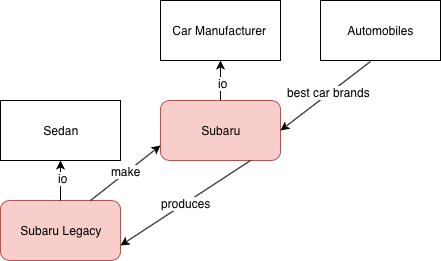
\includegraphics[width=4in]{sample_ontology}
\caption{This sample ontology, with inspiration from an example by Natalya F. Noy, describes entities and relations in the 'automobiles' domain. The ontology serves to provide a "formal explicit description" of classes (outlined in black) along with properties which describe relationships between classes (such as how Subaru Legacy is produced by Subaru). While not displayed in the figure, an ontology also defines property restrictions within the domain (so an instance of the Subaru class cannot produce a car manufacturer). The ontology, along with individual instances of classes (highlighted in red) constitutes a knowledge base \cite{noy2001ontology}. }
\label{fig:sample_ontology}
\end{figure}

In reality, few differences between an ontology and a knowledge base exists. Knowledge engineers must traverse a "fine line where the ontology ends and the knowledge base begins" \cite{noy2001ontology}. At the least, an ontology defines categories (or classes) and relationships among objects. One can think of an ontology as a "vocabulary" used to describe a domain \cite[308]{russell2016artificial}. Typically, both classes and relationships between classes can be arranged as hierarchies  (see Figure \ref{fig:sample_ontology}), which are here referred to as semantic hierarchies. When designing an ontology, one must decide the scope and organization of the knowledge, along with the language used. 

\subsubsection{Class Inheritance and Semantic Reasoning}

Many relations within an ontology serve to organize classes. For example, in the 'automobiles' ontology, most of the classes are organized by "is-a" relationships and classes inherit attributes such as domain and range restrictions. For example, my car would inherit properties of the 'Automobile', 'Sedan', and 'Subaru Legacy' classes, such as having four seats. 

\begin{figure}[h]
\centering
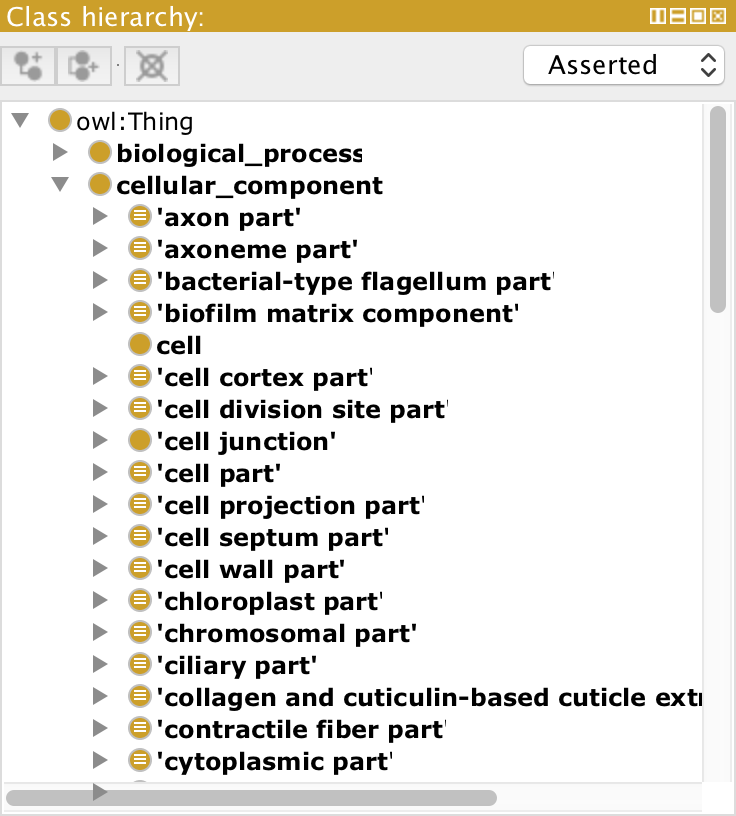
\includegraphics[width=2.5in]{class-hierarchy}
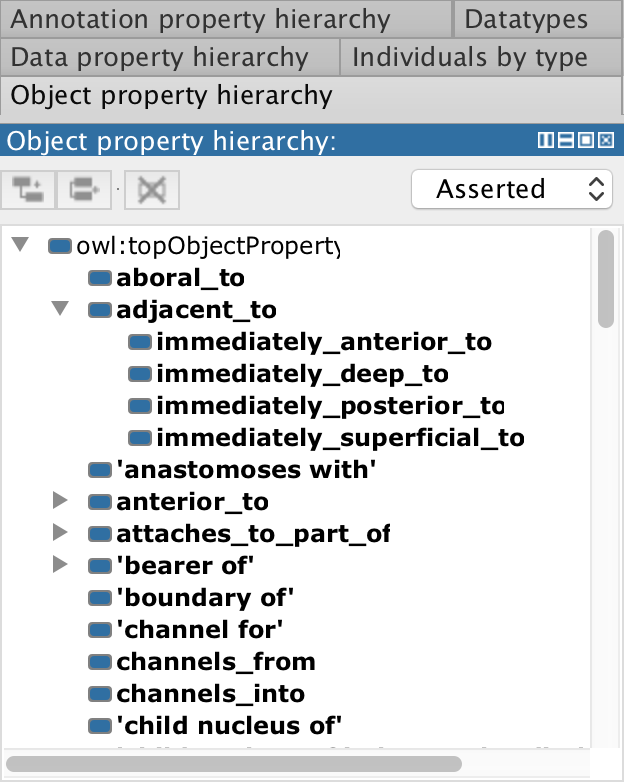
\includegraphics[width=2.5in]{object-property-hierarchy}
\caption{Hierarchies describing classes and relationships within the commonly used Gene Ontology (not used for experiments)  can be viewed in Prot{\'e}g{\'e}, with inferred hierarchies generated by Pellet reasoner \cite{gennari2003evolution}.}
\label{fig:class-hierarchy}
\end{figure}

Software tools referred to as semantic reasoners, or simply reasoners, can infer logical consequences from a set of axioms. Because an ontology may not explicitly define all relationships between classes and properties, one may use a reasoner to deduce implicit knowledge. A reasoner can generate a more complete view of an ontology, specifically complete hierarchies describing classes and relationships. These hierarchies are referred to as semantic hierarchies. 

Ontologies, especially those used in research, can contain hundreds or thousands of classes and relationships but only a small fraction of those are likely needed for any specific proof. By consulting knowledge embedded in the semantic hierarchies for a specific ontology one could possibly reduce the time needed to prove a specific conjecture when many irrelevant axioms exist. 

\subsubsection{First-order Logic Ontologies}

Automatic theorem proving requires a logic defining the syntax of valid statements to run without additional user input. Formal logics like first-order logic, also known as predicate logic and first-order predicate calculus, define a structure for statements which can be used to form logical and mathematical proofs. Consider the following set of asserted facts expressed in first-order predicate logic, commonly referred to as axioms. 

\begin{singlespace}
\[isSedan(Subaru Legacy)\]
\[\forall x \; isSedan(x) \rightarrow hasFourSeats(x)\]
\end{singlespace} 

The first axiom asserts the Subaru Legacy is a sedan. The second axiom asserts all sedans have four seats. By expressing facts in a formal notation, one makes proofs using such statements mechanical and easily parsed by a computer. Ontologies used for experiments are described used Common Logic, a formal logic based on first-order logic. Predicates describe objects in a knowledge base. In the cases above, $isSedan()$ would serve as a predicate acting on a $SubaruLegacy$ object in the former, and a variable labeled $x$ in the latter. Variables in first-order logic are quantified, meaning the application of a variable is defined for either some ($\exists$) or all ($\forall$) objects in the domain. 

\subsection{{Theorem Proving}}
Automated theorem proving depends on having an established logic for expressing facts (such as Common Logic), a method of generating new facts without requiring additional knowledge, and a strategy for searching through all possible new facts one could generate to reach a specific goal (such as proving a conjecture).

\subsubsection{Inference Rules}

One can use axioms to derive facts which logically follow using inference rules. The two previous statements do not directly state the Subaru Legacy has four seats. However, one can derive the statement $hasFourSeats(Subaru Legacy)$ by using the inference rule \textit{modus ponens}, defined below. 
\begin{equation}
\begin{gathered}
A \\
\frac{A \rightarrow B}{\therefore B}
\end{gathered}
\end{equation}

One can think of $A$ and $B$ as variables representing statements, and any statements can replace them. In the example above, one can replace $A$ with $isSedan(Subaru Legacy)$ and B with $hasFourSeats(SubaruLegacy)$ after instantiating $x$ with $Subaru Legacy$ (which is possible because $x$ is bound by the universal quantifier $\forall$ and we can replace $x$ with anything defined in the domain). Therefore, one can assert $hasFourSeats(Subaru Legacy)$ is true, without the statement having been defined explicitly as an axiom. An inference rule defines a valid rule for statements and always generates true statements when the assumed premises are true. 
\subsubsection{Resolution}

Automated theorem proving requires a set of axioms and a set of rules to generate new facts, but also a strategy to search through the possible applications of the inference rules. Knowledge bases can grow quite large, and generating all possible facts based on a given set of axioms often remains impractical or unfeasible. Resolution exists as historically significant and widely used method for automated theorem proving \cite[51]{ertel2018introduction}. 

\begin{figure}[h]
\centering
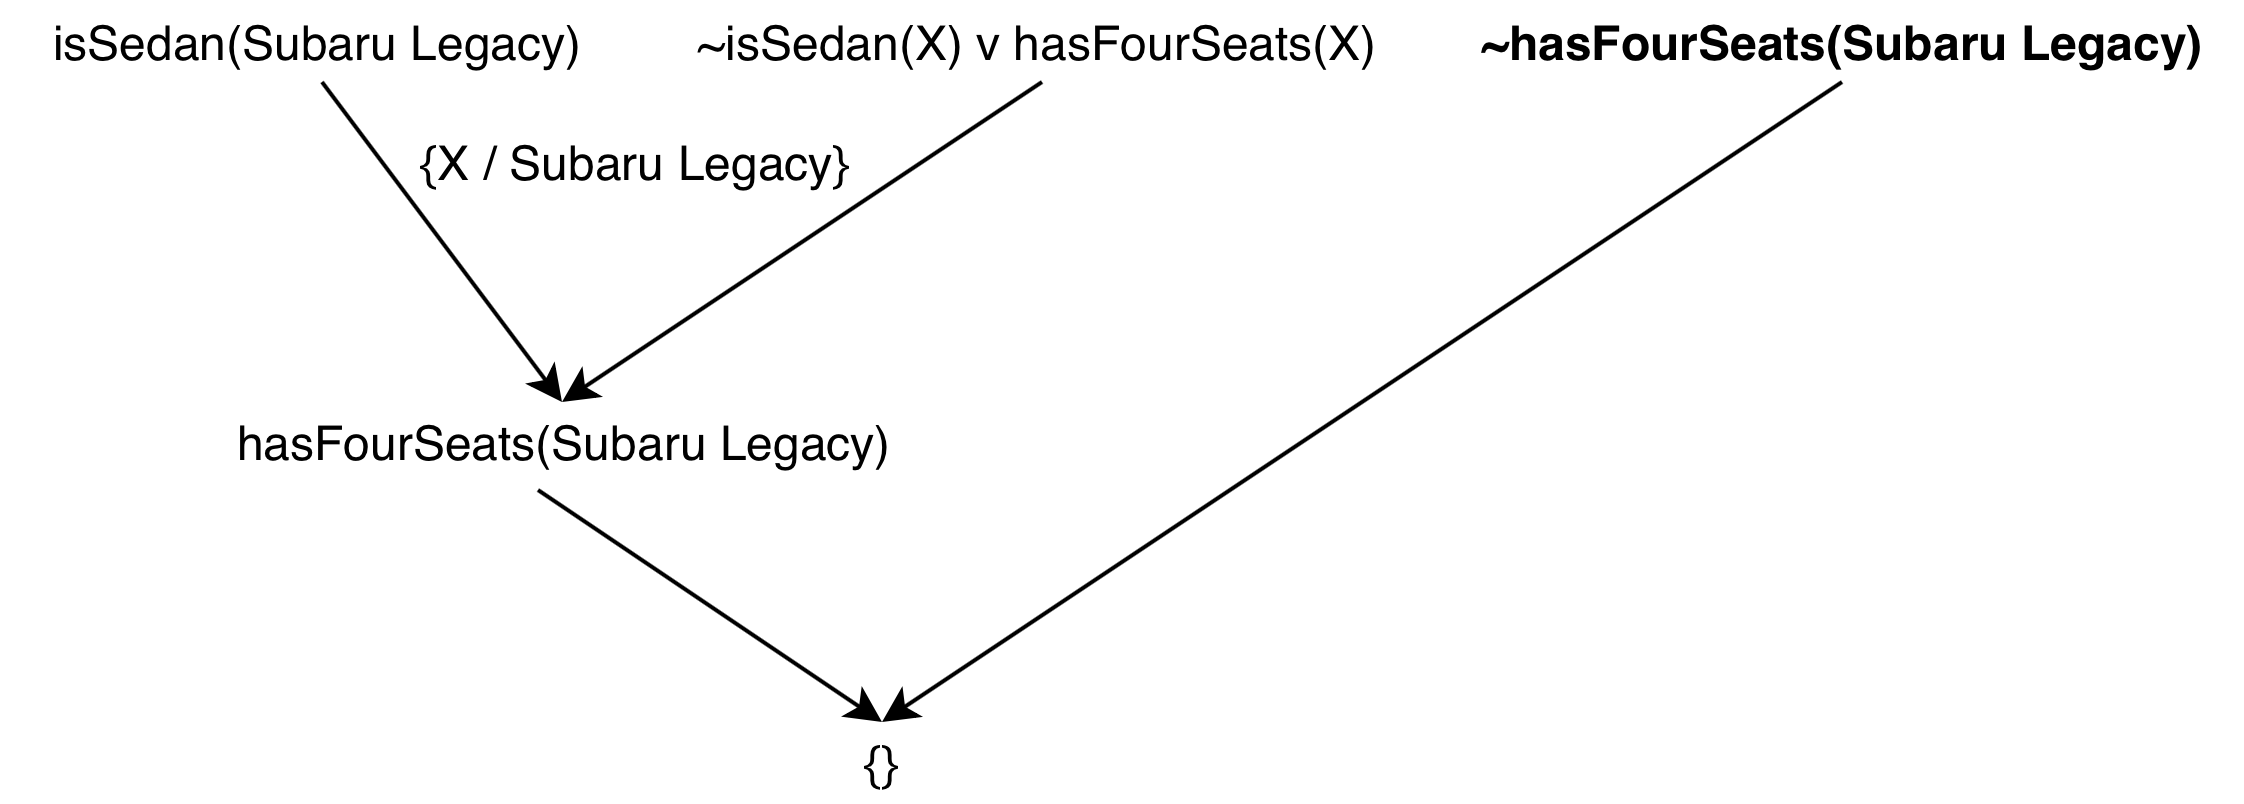
\includegraphics[width=6in]{resolution_tree}
\caption{The figure above displays a resolution tree for the inference rule described in the previous section. The bold statement shows the negated conjecture. The tree also displays $x$ bound to $SubaruLegacy$.}
\label{fig:resolution_tree}
\end{figure}

In order to use resolution as a proof technique, axioms must first be expressed in Conjunctive Normal Form (CNF), also known as clausal form. One may follow a 7-step procedure of converting the set of facts into a conjunction of disjunctions. The process eliminates biconditionals, implications, and quantifiers so the second axiom $\forall x \; isSedan(x) \rightarrow hasFourSeats(x)$ becomes 
$\lnot isSedan(x) \lor hasFourSeats(x)$. One can then resolve the statements by instantiating the variable $x$ with $SubaruLegacy$ in a process called unification, binding the variable. 
\[\frac{isSedan(Subaru Legacy), \lnot isSedan(x) \lor hasFourSeats(x)}{hasFourSeats(Subaru Legacy)}\]
Finally, one can resolve the axiom with the negated conjecture, proving the statement true. 

\begin{figure}[h]
\begin{verbatim}
1 (all x (isSedan(x) -> hasFourSeats(x))) # label(non_clause).  [assumption].
2 hasFourSeats(SubaruLegacy) # label(non_clause) # label(goal).  [goal].
3 -isSedan(x) | hasFourSeats(x).  [clausify(1)].
4 isSedan(SubaruLegacy).  [assumption].
5 hasFourSeats(SubaruLegacy).  [resolve(3,a,4,a)].
6 -hasFourSeats(SubaruLegacy).  [deny(2)].
7 $F.  [resolve(5,a,6,a)].
\end{verbatim}
\caption{Prover9 displays output for the automated proof. }
\label{fig:prover9out}
\end{figure}

Because the number of clauses an automated theorem prover can generate greatly increases with respect to the size of the knowledge base, researchers have begun to form heuristics to evaluate the relevance of axioms when completing a proof. Some methods include evaluating the semantic similarity between predicates to determine which axioms might be more relevant when attempting to form a proof. 

\subsection{Semantic Similarity}
Evaluating the similarity of two entities (i.e. classes or relationships) can serve as one heuristic when attempting to reduce the number of clauses generated during a proof. Multiple metrics have been developed for evaluating the semantic similarity of terms with different approaches, including: edge-counting measures, feature-based measures, and measures based on Information Content \cite{sanchez2012ontology} \cite{rodriguez1999assessing} \cite{roederer2009divvy}.  Edge-counting metrics for semantic similarity when applied to semantic hierarchies remain the focus of this work. 

Calculating the distance between two entities in an ontology is a a straightforward and intuitive method of calculating the semantic similarity. One can formally define the metric as follows. In an undirected graph $G$ defined as a pair $(V,E)$, where $V$ is a set of vertices, and $E$ is a set of edges between the vertices $E \subseteq {(u,v) | u, v \in V}$, one can define a path $path(a,b)=l_{1,\dots ,}l_k$ as a set of links connecting $a$ and $b$ in a taxonomy and $\lvert path(a,b) \rvert = k$ as the length of the path \cite{sanchez2012ontology}. One can calculate the semantic distance between $a$ and $b$ using equation \ref{rada} \cite{rada1989development}.

\begin{equation}
sim_1(a,b)=min_{\forall i}\lvert{path_i(a,b)}\rvert
\label{rada}
\end{equation}
Semantic hierarchies can be expressed as trees, and by incorporating depth of the taxonomy into the function, Zhibiao Wu has seen improvement in the metric. Because ontologies can vary greatly in depth due to the design of the ontology, some researchers have attempted to calculate semantic similarity using the lowest common ancestor (LCA), defined between two verticies $a$ and $b$ as the lowest vertex in the tree with both $a$ and $b$ as descendants (where we allow a vertex to be a descendant of itself) \cite{wu1994verbs}. The $root$ of a tree has no ancestors. 
\begin{equation}
sim_2(a,b)=\frac{2 \times sim_1(LCA,root)}{sim_1(a,LCA)+sim_1(b,LCA)+2 \times sim_1(LCA,root)}
\label{wu}
\end{equation}

\newpage
\vspace*{.05in}
\section{\MakeUppercase{Approach}}
This work aims to evaluate the effectiveness of using a semantic hierarchy generated from an ontology to calculate weights for predicates that will help focus the theorem prover on using axioms that are deemed more relevant to proving a conjecture. In efforts to quantitatively evaluate the effectiveness of the proposed methods, a series of experiments are conducted on multiple ontologies from the COmmon Logic Ontology REpository (COLORE)\footnote{\url{https://code.google.com/p/colore}}, a "testbed for ontology evaluation and integration techniques" \cite{gruninger2012specifying}. Pellet, a semantic reasoner, is used to generate semantic hierarchies, which are then used to calculate the assigned weights for each predicate when executing proofs. Finally, tests were run using Prover9 to compare the default weights to the calculated weights. The effectiveness of the process was measured by comparing the number of clauses generated by Prover9 for each proof. 

\begin{figure}[h]
\centering
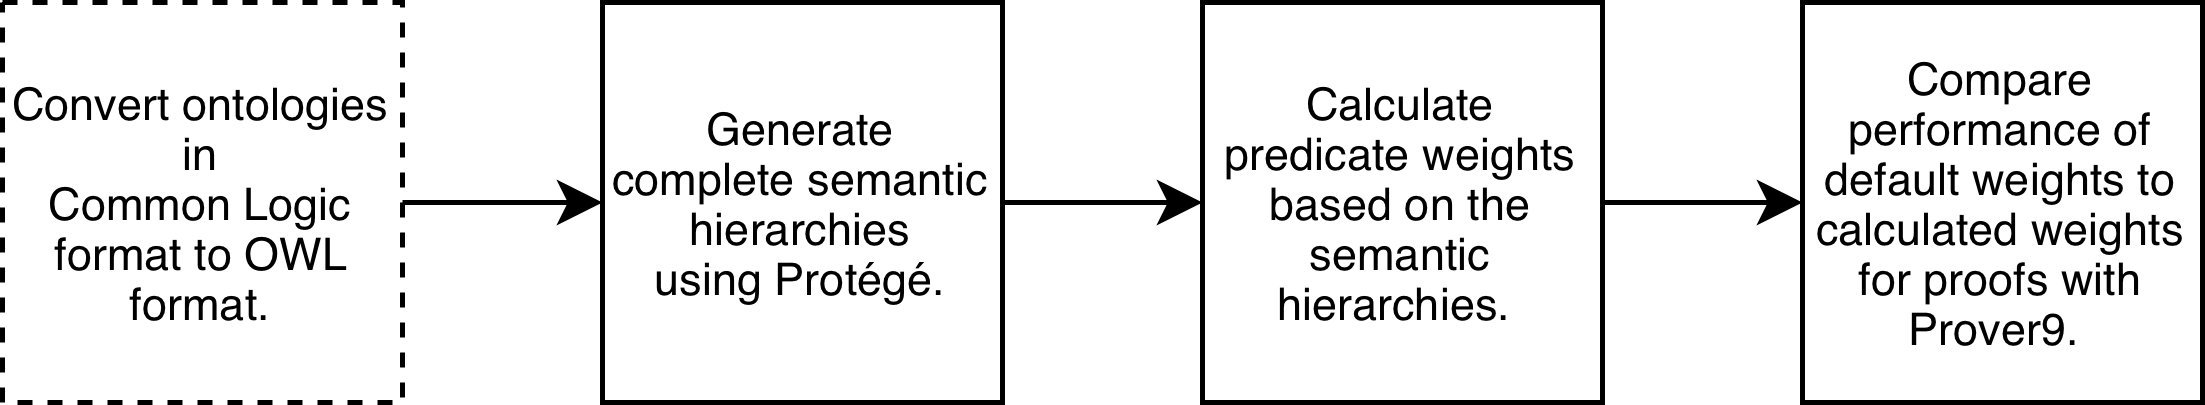
\includegraphics[width=6in]{flowchart}
\caption{The figure above illustrates my process of conducting experiments. The first step, converting the ontologies into OWL format, lives outside of the scope of my research.}
\label{fig:flowchart}
\end{figure}

\subsection{Converting Ontologies}
The ontologies in COLORE are specified using the Common Logic syntax. No tools exist for generation of the complete hierarchy directly from an ontology defined using Common Logic. However, virtually all Web Ontology Language (OWL) reasoners efficiently implement the task of organizing classes. Thus, one needs to translate the ontology to OWL, use an OWL reasoner to complete the hierarchy, and then calculate predicate weight based on that hierarchy. Robert Powell has written a utility which executes the conversion and has generated the files necessary to conduct this research. Not all ontologies in COLORE have conjectures, which limits the scope of my experiments to the sufficiently large ontologies. 

\subsection{Generating a Complete Heirarchy}
After converting an ontology into the OWL format, one can generate semantic heirarchies including both asserted relationships and inferred relationships. Pellet can be used to generate the inferred semantic hierarchy, which are then displayed in 
 Prot{\'e}g{\'e} (Figure \ref{fig:class-hierarchy}). The reasoner parses the axioms for inferred logical consequences (i.e. relationships between classes) not explicitly defined. The reasoner generates complete class hierarchies, but does not change the relationship hierarchy.

\subsection{Calculating Weights for Resolution Theorem Proving}
\subsubsection{Default Weights in Prover9}
Prover9 assigns weights to predicates automatically unless the user explicitly defines them. An understanding of the process helps one to develop new weights for the predicates. Lower weights give higher preference for a predicate when generating clauses. Rules for weighting axioms in terms of relevance when attempting to prove a specific conjecture are as follows \cite{mccune2005prover9}: 

\begin{singlespace}
\centering
\begin{itemize}
    \item The default weight of a constant or variable is 1.
    \item The default weight of a term or atomic formula is one more than the sum of the weights of its arguments.
    \item The default weight of a literal is the weight of its atomic formula.
    \item The default weight of a clause is the sum of the weights of its literals.
\end{itemize}
\end{singlespace}

Below is an example of how one may modify weights in Prover9  \cite{mccune2005prover9}. 

\begin{singlespace}
\centering
\begin{verbatim}
list(weights).
  weight(a) = 3.                               % the weight of the constant a is 3
  weight(f(a,x)) = 5 * weight(x).              % weight(f(a,term)) = 5 * weight(term)
  weight(f(a,_)) = -1.                         % _ matches any variable
  weight(x | y) = 2 + (weight(x) + weight(y)). % add 2 for each "or" symbol
end_of_list.
\end{verbatim}
\end{singlespace}

\subsubsection{Semantic Weighting Functions}
Assigning weights to specific predicates will likely yield the best results. After semantic hierarchies have been generated, weights can be assigned to each class and subproperty. Two explicit weighting functions inspired by related works in calculating semantic similarity, were formed and tested. The weights for each conjecture were then calculated by hand and entered into a spreadsheet. A python script was used to generate the input files used by Prover9 from the spreadsheet for each conjecture. The calculated weights were then entered into Prover9 as additional input along with the axioms and the conjecture. The weighting functions are currently applied by hand to the ontologies, with the beginnings of an automated program underway. 

\subsubsection{Function 1} 

The first function attempts to make use of the completed class hierarchy generated by a semantic reasoner by giving preference to predicates existing on a path between pairs of predicates in the conjecture. For example, if one wished to prove the conjecture $Automobile(myCar)$ using the ontology provided in Figure \ref{fig:sample_ontology}, it is reasonable to assume the theorem prover would need to traverse a series of axioms ascending the class hierarchy. Also, the 'Sedan' and 'Subaru Legacy' classes might not be given as much preference as predicates contained in the conjecture (i.e. $Automobile(x)$). Additionally, if the conjecture contains relationships (such as $Produces(x,y)$), once can apply the same principles. Additionally, in efforts to give lower preference to predicates not contained on paths connecting pairs of classes or relationships, unweighted ancestors and descendants are assigned higher weights. In order to achieve the goals above, Function 1 is defined as follows: 

\begin{singlespace}
\begin{itemize}
	\item Each predicate describing a class or relationship contained in the conjecture is given weight 1. 
	\item For each pair of predicates describing classes within the conjecture, if a path exists between the two classes in the class hierarchy, predicates describing classes contained on the path are given weight 1. 
	\item For each pair of predicates describing relationships within the conjecture, if a path exists between the two relationships in the relationship hierarchy, predicates describing relationships contained on the path are given weight 1. 
	\item Decedents of predicates describing classes or relationships contained in conjecture without weights are given a weight corresponding to the depth of the entity. Subclasses and sub-properties are given a weight of the respective parent class or property plus 1. 
	\item All ancestors of predicates with a weight generated and all top-level classes corresponding to predicates without a weight assigned are given weight 10.
	\item All ancestors of predicates with a weight generated all top-level relationships corresponding to predicates without a weight assigned are given weight 10.
\end{itemize}
\end{singlespace}

Given the example 'automobile' ontology and the conjecture $Automobile(myCar)$, the weights can be calculated as follows. 

\begin{singlespace}
\begin{verbatim}
list(weights).
  weight(SubaruLegacy(x)) = 1. 
  weight(Sedan(x)) = 1. 
  weight(Automobile(x)) = 1. 
  weight(Minivan(x)) = 2. 
  weight(ToyotaSienna(x)) = 3. 
  weight(FordWindstar(x)) = 3. 
  weight(CarManufactuer(x)) = 10. 
  % weight(Produces(x,y)) - This is not defined as the conjecture contains no relationships. 
end_of_list.
\end{verbatim}
\end{singlespace}

\subsubsection{Function 2}

The second function attempts to make use of the lowest common ancestor (LCA) of each class or relationship with inspiration from equation \ref{wu}. Again, predicates in within the conjecture are preferred. Siblings and the parent of the LCA are weighted highly, and decedents of predicates without weights are given weights increasing with the depth of the semantic hierarchy. 

\begin{singlespace}
\begin{itemize}
	\item Each predicate describing a class or relationship contained in the conjecture is given weight 1. 
	\item For each pair of predicates describing classes within the conjecture, if a path exists between the two classes in the class hierarchy, predicates describing the lowest common ancestor are given weight 1 and classes contained on the path which are neither a predicate contained in the conjecture or the lowest common ancestor are given weight 2. 
	\item For each pair of predicates describing relationships within the conjecture, if a path exists between the two relationships in the class hierarchy, predicates describing the lowest common ancestor are given weight 1 and classes contained on the path which are neither a predicate contained in the conjecture or the lowest common ancestor are given weight 2. 
	\item Siblings and parents of a LCA are given a weight 3. 
	\item Decedents of predicates describing classes or relationships contained in conjecture without weights are given a weight corresponding to the depth of the entity. Subclasses and sub-properties are given a weight of the respective parent class or property plus 1. 
\end{itemize}
\end{singlespace}

Given the example 'automobile' ontology and the conjecture $FordWindstar(myCar) \lor SubaruLegacy(myCar)$,   the weights can be calculated as follows. 

\begin{singlespace}
\begin{verbatim}
list(weights).
  weight(SubaruLegacy(x)) = 1. 
  weight(FordWindstar(x)) = 1. 
  weight(Automobile(x)) = 1. % LCA
  weight(Sedan(x)) = 2. 
  weight(Minivan(x)) = 2. 
  weight(ToyotaSienna(x)) = 3. 
  weight(CarManufactuer(x)) = 3. 
end_of_list.
\end{verbatim}
\end{singlespace}

\newpage
\vspace*{.05in}
\section{\MakeUppercase{Experiments}}

\subsection{{Setup}}

Experiments were conducted using Prover9, an "automated theorem prover for first-order and equational logic" written by William McCune \cite{mccune2005prover9}. Many tests were conducted using a version of the program which supports a Graphical User Interface (GUI), but a command line version, useful for running automated tests, exists. 
Git was used for version control and a repository containing source code for tests can be found at \url{https://github.com/stanleysmall/thesis}.
\begin{figure}[h]
\centering
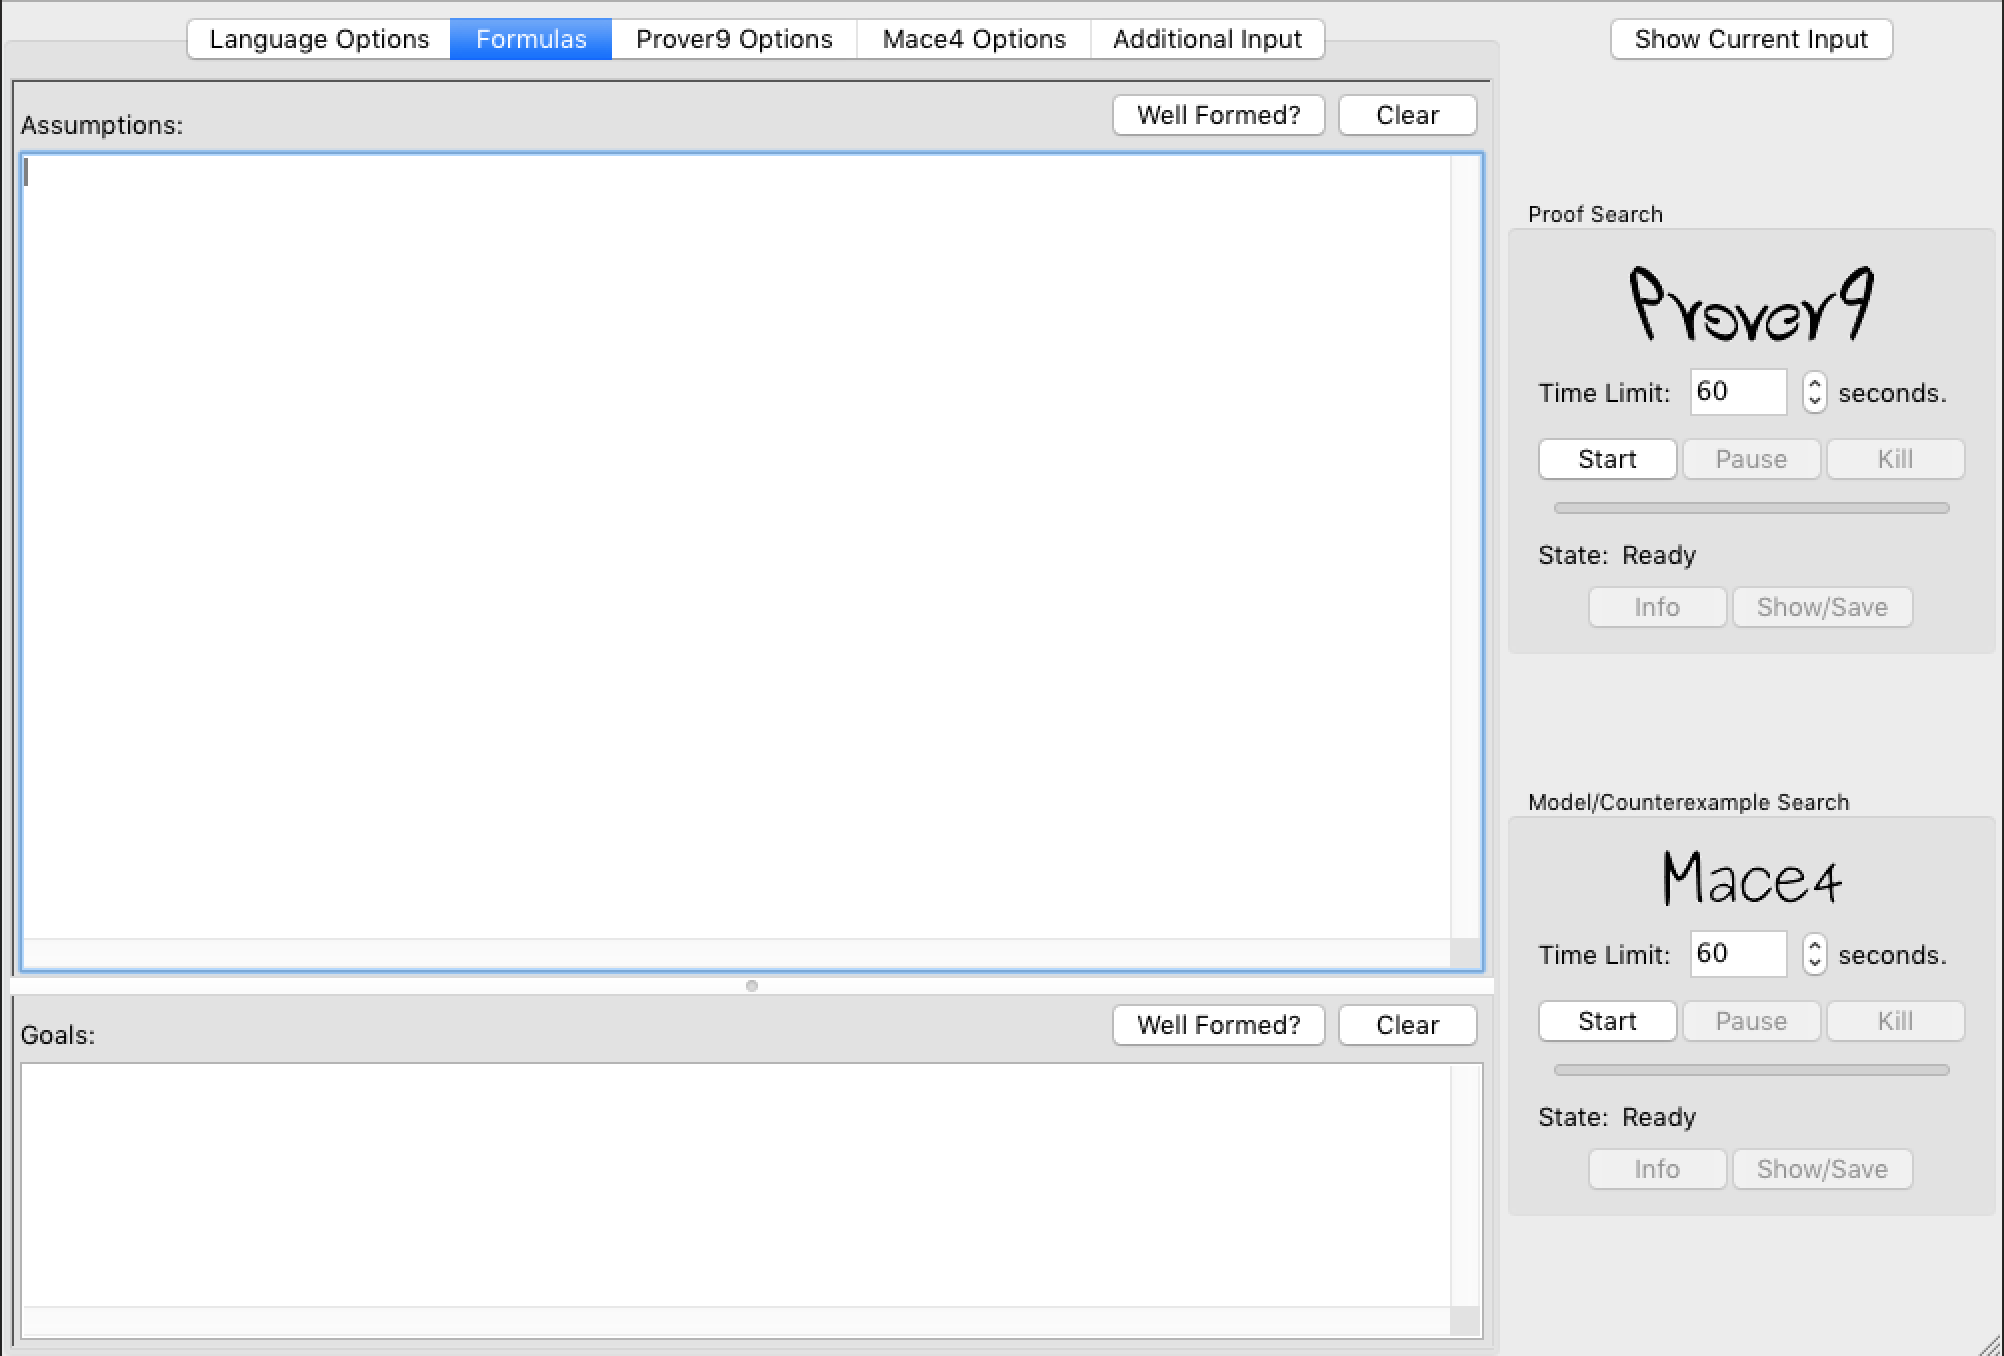
\includegraphics[width=6in]{prover9}
\caption{The GUI for Prover9 on macOS is shown above. One enters axioms into the top text field and conjectures into the bottom text field. Predicate weights are entered in the 'Additional Input' tab in the navigation bar. Users can start the proof by pressing the 'Start' button below the Prover9 logo after specifying a time limit. After the proof has completed, users can view the number of clauses generated by the proof by pressing the 'Info' button below the 'Start' button \cite{mccune2005prover9}.}
\label{fig:prover9}
\end{figure}

\subsection{Results}
\subsubsection{multidim\_space\_voids}
\begin{table}[h]
\centering
\csvautotabular{tests/multidim_space_voids/results.csv}
\caption{Results for the multidim\_space\_voids Ontology}
\end{table}

\subsubsection{inch}
\begin{table}[h]
\centering
\csvautotabular{tests/inch/results.csv}
\caption{Results for the inch Ontology}
\end{table}

\subsection{Discussion}

\newpage
\vspace*{.05in}
\section{\MakeUppercase{Conclusion}}

In some cases, the algorithm increases the number of clauses generated for each test, but does not do so to the point where the tests are unusable. For the majority of proofs, the number of clauses generated decreases or remains unchanged.

The scarcity of suitable ontologies to test provides many opportunities for advancement. 

Many opportunities for further research include fully automating the search procedure, working with a larger number of ontologies to ensure the weighting functions actually do as they say, developing a new approach towards automatically weighting the predicates. 
\newpage
\addcontentsline{toc}{section}{\MakeUppercase{References}}
\vspace*{.05in}
\printbibliography

\newpage
\appendix
\section{\MakeUppercase{Tests}}
\begin{singlespace}
\csvautolongtable[
      table head=\caption{multidim space voids weights for function 1}\label{tab:some}\\\hline
               \csvlinetotablerow\\\hline
               \endfirsthead\hline
               \csvlinetotablerow\\\hline
               \endhead\hline
               \endfoot,
               respect all
               ]{tests/multidim_space_voids/weights1.csv}
               
\csvautolongtable[
      table head=\caption{multidim space voids weights for function 2}\label{tab:some}\\\hline
               \csvlinetotablerow\\\hline
               \endfirsthead\hline
               \csvlinetotablerow\\\hline
               \endhead\hline
               \endfoot,
               respect all
               ]{tests/multidim_space_voids/weights2.csv}
               
\csvautolongtable[
      table head=\caption{inch weights for function 1}\label{tab:some}\\\hline
               \csvlinetotablerow\\\hline
               \endfirsthead\hline
               \csvlinetotablerow\\\hline
               \endhead\hline
               \endfoot,
               respect all
               ]{tests/inch/weights1.csv}
               
\csvautolongtable[
      table head=\caption{inch weights for function 2}\label{tab:some}\\\hline
               \csvlinetotablerow\\\hline
               \endfirsthead\hline
               \csvlinetotablerow\\\hline
               \endhead\hline
               \endfoot,
               respect all
               ]{tests/inch/weights2.csv}
               
               
\end{singlespace}


\newpage
\addcontentsline{toc}{section}{\MakeUppercase{Author's Biography}}
\vspace*{.05in}
\section*{\MakeUppercase{Author's Biography}}
Stanley C. Small grew up in Hampden, Maine with his mother Diane and his father Scott. He attended the University of Maine and received a Bachelor of Science degree in Computer Science in May of 2019. 


\end{document}
